\documentclass[journal,12pt,twocolumn]{IEEEtran}
\usepackage{setspace}
\usepackage{gensymb}
\usepackage{caption}
%\usepackage{multirow}
%\usepackage{multicolumn}
%\usepackage{subcaption}
%\doublespacing
\singlespacing
\usepackage{csvsimple}
\usepackage{amsmath}
\usepackage{multicol}
\usepackage{enumerate}
\usepackage{amssymb}
\usepackage{graphicx}
\usepackage{newfloat}
%\usepackage{syntax}
\usepackage{listings}
%\usepackage{iithtlc}
\usepackage{color}
\usepackage{tikz}
\usetikzlibrary{shapes,arrows}



%\usepackage{graphicx}
%\usepackage{amssymb}
%\usepackage{relsize}
%\usepackage[cmex10]{amsmath}
%\usepackage{mathtools}
%\usepackage{amsthm}
%\interdisplaylinepenalty=2500
%\savesymbol{iint}
%\usepackage{txfonts}
%\restoresymbol{TXF}{iint}
%\usepackage{wasysym}
\usepackage{amsthm}
\usepackage{mathrsfs}
\usepackage{txfonts}
\usepackage{stfloats}
\usepackage{cite}
\usepackage{cases}
\usepackage{mathtools}
\usepackage{caption}
\usepackage{enumerate}	
\usepackage{enumitem}
\usepackage{amsmath}
%\usepackage{xtab}
\usepackage{longtable}
\usepackage{multirow}
%\usepackage{algorithm}
%\usepackage{algpseudocode}
\usepackage{enumitem}
\usepackage{mathtools}
\usepackage{hyperref}
%\usepackage[framemethod=tikz]{mdframed}
\usepackage{listings}
    %\usepackage[latin1]{inputenc}                                 %%
    \usepackage{color}                                            %%
    \usepackage{array}                                            %%
    \usepackage{longtable}                                        %%
    \usepackage{calc}                                             %%
    \usepackage{multirow}                                         %%
    \usepackage{hhline}                                           %%
    \usepackage{ifthen}                                           %%
  %optionally (for landscape tables embedded in another document): %%
    \usepackage{lscape}     


\usepackage{url}
\def\UrlBreaks{\do\/\do-}


%\usepackage{stmaryrd}


%\usepackage{wasysym}
%\newcounter{MYtempeqncnt}
\DeclareMathOperator*{\Res}{Res}
%\renewcommand{\baselinestretch}{2}
\renewcommand\thesection{\arabic{section}}
\renewcommand\thesubsection{\thesection.\arabic{subsection}}
\renewcommand\thesubsubsection{\thesubsection.\arabic{subsubsection}}

\renewcommand\thesectiondis{\arabic{section}}
\renewcommand\thesubsectiondis{\thesectiondis.\arabic{subsection}}
\renewcommand\thesubsubsectiondis{\thesubsectiondis.\arabic{subsubsection}}

% correct bad hyphenation here
\hyphenation{op-tical net-works semi-conduc-tor}

%\lstset{
%language=C,
%frame=single, 
%breaklines=true
%}

%\lstset{
	%%basicstyle=\small\ttfamily\bfseries,
	%%numberstyle=\small\ttfamily,
	%language=Octave,
	%backgroundcolor=\color{white},
	%%frame=single,
	%%keywordstyle=\bfseries,
	%%breaklines=true,
	%%showstringspaces=false,
	%%xleftmargin=-10mm,
	%%aboveskip=-1mm,
	%%belowskip=0mm
%}

%\surroundwithmdframed[width=\columnwidth]{lstlisting}
\def\inputGnumericTable{}                                 %%
\lstset{
%language=C,
frame=single, 
breaklines=true,
columns=fullflexible
}
 

\begin{document}
%
\tikzstyle{block} = [rectangle, draw,
    text width=3em, text centered, minimum height=3em]
\tikzstyle{sum} = [draw, circle, node distance=3cm]
\tikzstyle{input} = [coordinate]
\tikzstyle{output} = [coordinate]
\tikzstyle{pinstyle} = [pin edge={to-,thin,black}]

\theoremstyle{definition}
\newtheorem{theorem}{Theorem}[section]
\newtheorem{problem}{Problem}
\newtheorem{proposition}{Proposition}[section]
\newtheorem{lemma}{Lemma}[section]
\newtheorem{corollary}[theorem]{Corollary}
\newtheorem{example}{Example}[section]
\newtheorem{definition}{Definition}[section]
%\newtheorem{algorithm}{Algorithm}[section]
%\newtheorem{cor}{Corollary}
\newcommand{\BEQA}{\begin{eqnarray}}
\newcommand{\EEQA}{\end{eqnarray}}
\newcommand{\define}{\stackrel{\triangle}{=}}

\bibliographystyle{IEEEtran}
%\bibliographystyle{ieeetr}

\providecommand{\nCr}[2]{\,^{#1}C_{#2}} % nCr
\providecommand{\nPr}[2]{\,^{#1}P_{#2}} % nPr
\providecommand{\mbf}{\mathbf}
\providecommand{\pr}[1]{\ensuremath{\Pr\left(#1\right)}}
\providecommand{\qfunc}[1]{\ensuremath{Q\left(#1\right)}}
\providecommand{\sbrak}[1]{\ensuremath{{}\left[#1\right]}}
\providecommand{\lsbrak}[1]{\ensuremath{{}\left[#1\right.}}
\providecommand{\rsbrak}[1]{\ensuremath{{}\left.#1\right]}}
\providecommand{\brak}[1]{\ensuremath{\left(#1\right)}}
\providecommand{\lbrak}[1]{\ensuremath{\left(#1\right.}}
\providecommand{\rbrak}[1]{\ensuremath{\left.#1\right)}}
\providecommand{\cbrak}[1]{\ensuremath{\left\{#1\right\}}}
\providecommand{\lcbrak}[1]{\ensuremath{\left\{#1\right.}}
\providecommand{\rcbrak}[1]{\ensuremath{\left.#1\right\}}}
\theoremstyle{remark}
\newtheorem{rem}{Remark}
\newcommand{\sgn}{\mathop{\mathrm{sgn}}}
\providecommand{\abs}[1]{\left\vert#1\right\vert}
\providecommand{\res}[1]{\Res\displaylimits_{#1}} 
\providecommand{\norm}[1]{\left\Vert#1\right\Vert}
\providecommand{\mtx}[1]{\mathbf{#1}}
\providecommand{\mean}[1]{E\left[ #1 \right]}
\providecommand{\fourier}{\overset{\mathcal{F}}{ \rightleftharpoons}}
%\providecommand{\hilbert}{\overset{\mathcal{H}}{ \rightleftharpoons}}
\providecommand{\system}{\overset{\mathcal{H}}{ \longleftrightarrow}}
	%\newcommand{\solution}[2]{\textbf{Solution:}{#1}}
\newcommand{\solution}{\noindent \textbf{Solution: }}
\newcommand{\myvec}[1]{\ensuremath{\begin{pmatrix}#1\end{pmatrix}}}
\providecommand{\dec}[2]{\ensuremath{\overset{#1}{\underset{#2}{\gtrless}}}}
\DeclarePairedDelimiter{\ceil}{\lceil}{\rceil}
%\numberwithin{equation}{section}
%\numberwithin{problem}{subsection}
%\numberwithin{definition}{subsection}
\makeatletter
\@addtoreset{figure}{section}
\makeatother

\let\StandardTheFigure\thefigure
%\renewcommand{\thefigure}{\theproblem.\arabic{figure}}
\renewcommand{\thefigure}{\thesection}


%\numberwithin{figure}{subsection}

%\numberwithin{equation}{subsection}
%\numberwithin{equation}{section}
%\numberwithin{equation}{problem}
%\numberwithin{problem}{subsection}
\numberwithin{problem}{section}
%%\numberwithin{definition}{subsection}
%\makeatletter
%\@addtoreset{figure}{problem}
%\makeatother
\makeatletter
\@addtoreset{table}{section}
\makeatother

\let\StandardTheFigure\thefigure
\let\StandardTheTable\thetable
\let\vec\mathbf
\numberwithin{equation}{section}

\vspace{3cm}


\title{%Convex Optimization in Python
	\logo{
	Random Numbers
	}
}
%\title{
%	\logo{Matrix Analysis through Octave}{\begin{center}\includegraphics[scale=.24]{tlc}\end{center}}{}{HAMDSP}
%}


% paper title
% can use linebreaks \\ within to get better formatting as desired
%\title{Matrix Analysis through Octave}
%
%
% author names and IEEE memberships
% note positions of commas and nonbreaking spaces ( ~ ) LaTeX will not break
% a structure at a ~ so this keeps an author's name from being broken across
% two lines.
% use \thanks{} to gain access to the first footnote area
% a separate \thanks must be used for each paragraph as LaTeX2e's \thanks
% was not built to handle multiple paragraphs
%

\author{ Pranav B% <-this % stops a space
% <-this % stops a space
%\thanks{J. Doe and J. Doe are with Anonymous University.}% <-this % stops a space
%\thanks{Manuscript received April 19, 2005; revised January 11, 2007.}}
}
% note the % following the last \IEEEmembership and also \thanks - 
% these prevent an unwanted space from occurring between the last author name
% and the end of the author line. i.e., if you had this:
% 
% \author{....lastname \thanks{...} \thanks{...} }
%                     ^------------^------------^----Do not want these spaces!
%
% a space would be appended to the last name and could cause every name on that
% line to be shifted left slightly. This is one of those "LaTeX things". For
% instance, "\textbf{A} \textbf{B}" will typeset as "A B" not "AB". To get
% "AB" then you have to do: "\textbf{A}\textbf{B}"
% \thanks is no different in this regard, so shield the last } of each \thanks
% that ends a line with a % and do not let a space in before the next \thanks.
% Spaces after \IEEEmembership other than the last one are OK (and needed) as
% you are supposed to have spaces between the names. For what it is worth,
% this is a minor point as most people would not even notice if the said evil
% space somehow managed to creep in.



% The paper headers
%\markboth{Journal of \LaTeX\ Class Files,~Vol.~6, No.~1, January~2007}%
%{Shell \MakeLowercase{\textit{et al.}}: Bare Demo of IEEEtran.cls for Journals}
% The only time the second header will appear is for the odd numbered pages
% after the title page when using the twoside option.
% 
% *** Note that you probably will NOT want to include the author's ***
% *** name in the headers of peer review papers.                   ***
% You can use \ifCLASSOPTIONpeerreview for conditional compilation here if
% you desire.




% If you want to put a publisher's ID mark on the page you can do it like
% this:
%\IEEEpubid{0000--0000/00\$00.00~\copyright~2007 IEEE}
% Remember, if you use this you must call \IEEEpubidadjcol in the second
% column for its text to clear the IEEEpubid mark.



% make the title area
\maketitle
\tableofcontents
\bigskip
\renewcommand{\thefigure}{\theenumi}
\renewcommand{\thetable}{\theenumi}
%%
\section{Uniform Random Numbers}
Let $U$ be a uniform random variable between 0 and 1.
\begin{enumerate}[label=\thesection.\arabic*
,ref=\thesection.\theenumi]
\item Generate $10^6$ samples of $U$ using a C program and save into a file called uni.dat .
\\
\solution Download the following files and execute the  C program.
\begin{lstlisting}
wget https://github.com/Pranavb060504/Random_numbers/blob/main/1.1/exrand.c
wget https://github.com/Pranavb060504/Random_numbers/blob/main/1.1/coeffs.h
\end{lstlisting}
Use the below command in the terminal to run the code
\begin{lstlisting}
cc exrand.c -lm
./a.out
\end{lstlisting}
\\
%
\item
Load the uni.dat file into python and plot the empirical CDF of $U$ using the samples in uni.dat. The CDF is defined as
\begin{align}
F_{U}(x) = \pr{U \le x}
\end{align}
\\
\solution 
The graph \ref{fig:uni_cdf} is obtained by running the below code
\begin{lstlisting}
https://github.com/Pranavb060504/Random_numbers/blob/main/1.2/uni_cdf.py
\end{lstlisting}
Run the following command in the terminal to run the code.\\
\begin{lstlisting}
python3 uni_cdf.py
\end{lstlisting}
\begin{figure}[h]
\centering
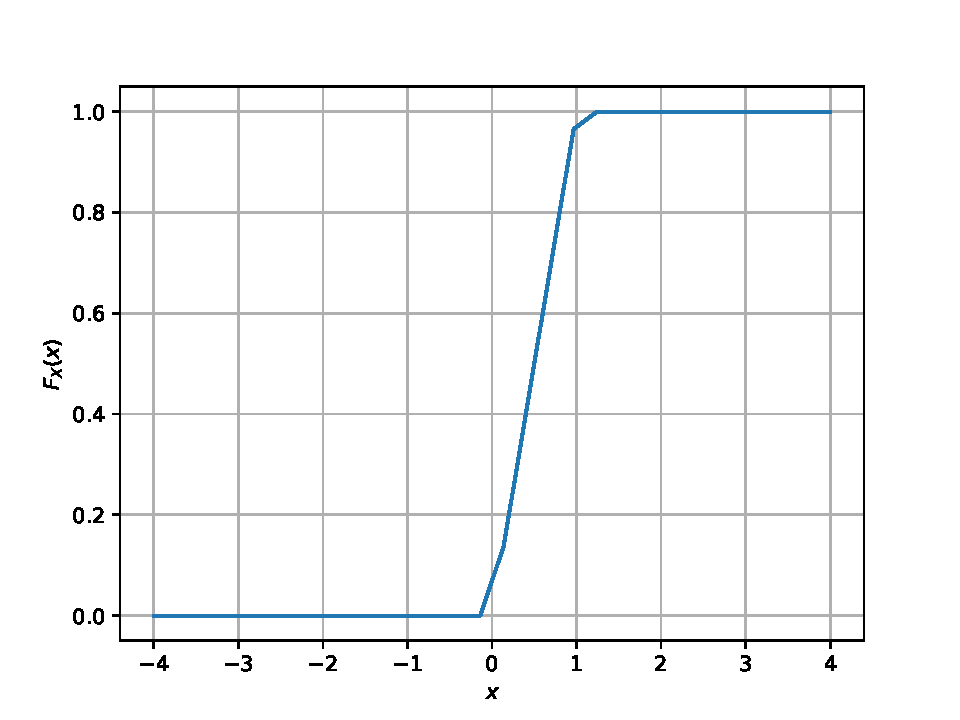
\includegraphics[width=\columnwidth]{./uni_cdf}
\caption{The CDF of $U$}
\label{fig:uni_cdf}
\end{figure}

%
\item
Find a  theoretical expression for $F_{U}(x)$.\\
\solution
Since U is an uniform random variable distribution, $P_{U}(x_{i})=P_{U}(x_{j})=k$,$\forall i,j$\\
	CDF of $P_{U}(x)$=$F_{U}(x)$\\
	\begin{align}
	=\int P_{U}(x) dx\\
	=\int k dx\\
  \text{wkt} \int_{0}^{1} kdx=1\\
  \therefore k=1\\
  \therefore F_{U}(x)=x
	\end{align}	
\item
The mean of $U$ is defined as
%
\begin{equation}
E\sbrak{U} = \frac{1}{N}\sum_{i=1}^{N}U_i
\end{equation}
%
and its variance as
%
\begin{equation}
\text{var}\sbrak{U} = E\sbrak{U- E\sbrak{U}}^2 
\end{equation}

Write a C program to  find the mean and variance of $U$. \\
\solution
\begin{lstlisting}
wget https://github.com/Pranavb060504/Random_numbers/blob/main/1.4/mean_var.c
\end{lstlisting}
Use below command to run file,
\begin{lstlisting}
cc mean_var.c -lm
./a.out
\end{lstlisting}
running the code gives us Mean =0.500137 , Variance =0.083251
\item Verify your result theoretically given that
\end{enumerate}
%
\begin{equation}
E\sbrak{U^k} = \int_{-\infty}^{\infty}x^kdF_{U}(x)
\end{equation}
\begin{align}
&dF_{U}(x)=dx\\
&\therefore E[U^k]=\int_{-\infty}^{\infty} x^k dx\\
&E[U]=\int_{0}^{1} x dx=\frac{1}{2}\\
&E[U^2]=\int_{0}^{1} x^2 dx=\frac{1}{3}\\
&\because P_{X}(x)=0 ,\forall x \in (1,\infty)\cap (-\infty,0)\\
&Var(X)=E[U^2]-(E[U])^2=\frac{1}{3}-\frac{1}{4}=\frac{1}{12}
\end{align}
\section{Central Limit Theorem}
%
\begin{enumerate}[label=\thesection.\arabic*
,ref=\thesection.\theenumi]

%
\item
Generate $10^6$ samples of the random variable
%
\begin{equation}
X = \sum_{i=1}^{12}U_i -6
\end{equation}
%
using a C program, where $U_i, i = 1,2,\dots, 12$ are  a set of independent uniform random variables between 0 and 1
and save in a file called gau.dat
\\
\solution
\begin{lstlisting}
wget https://github.com/Pranavb060504/Random_numbers/blob/main/1.1/exrand.c
wget https://github.com/Pranavb060504/Random_numbers/blob/main/1.1/coeffs.h
\end{lstlisting}
Running the above codes generates uni.dat and gau.dat file.
Use the command 
\begin{lstlisting}
cc exrand.c -lm
.\a.out
\end{lstlisting}
%
\item
Load gau.dat in python and plot the empirical CDF of $X$ using the samples in gau.dat. What properties does a CDF have?
\\
\solution 
The CDF of $X$ is plotted in \ref{fig:gau_cdf},Properties of the CDF:
\begin{itemize}
\item $\Phi(x)=P(Z \leq x)= \frac{1}{\sqrt{2 \pi}} \int_{-\infty}^{x}\exp\left\{-\frac{u^2}{2}\right\} du$
\item $\lim \limits_{x\rightarrow \infty} \Phi(x)=1, \hspace{5pt} \lim \limits_{x\rightarrow -\infty} \Phi(x)=0$
\item  $\Phi(0)=\frac{1}{2}$
\item  $\Phi(-x)=1-\Phi(x)$
\end{itemize}
\\
\begin{figure}[h]
\centering
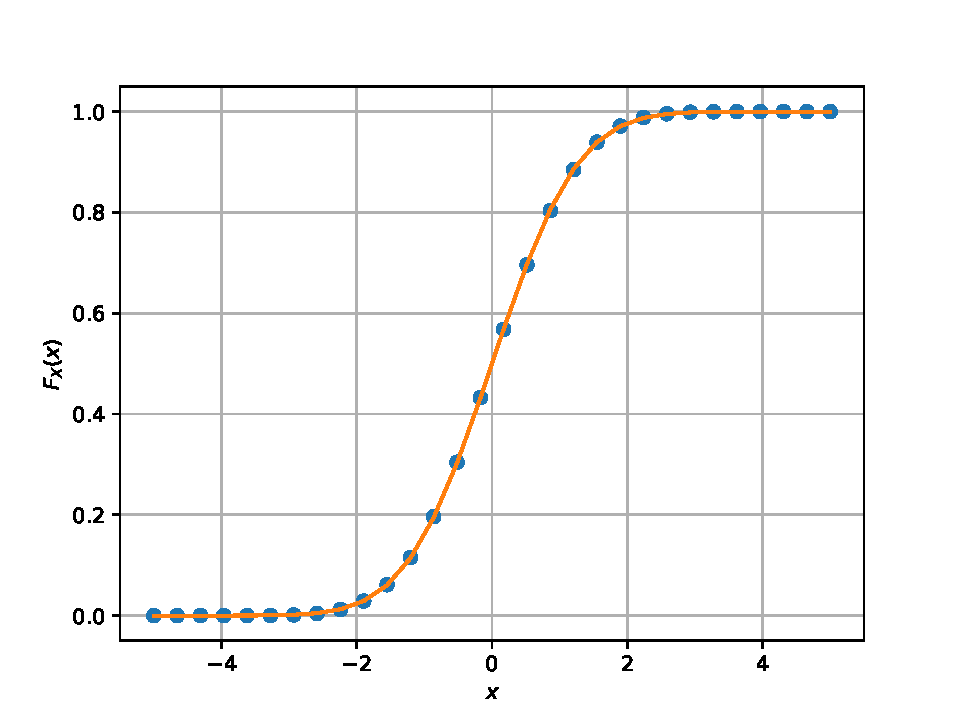
\includegraphics[width=\columnwidth]{./gau_cdf}
\caption{The CDF of $X$}
\label{fig:gau_cdf}
\end{figure}
\\
\item
Load gau.dat in python and plot the empirical PDF of $X$ using the samples in gau.dat. The PDF of $X$ is defined as
\begin{align}
p_{X}(x) = \frac{d}{dx}F_{X}(x)
\end{align}
What properties does the PDF have?
\\
\begin{figure}[h]
\centering
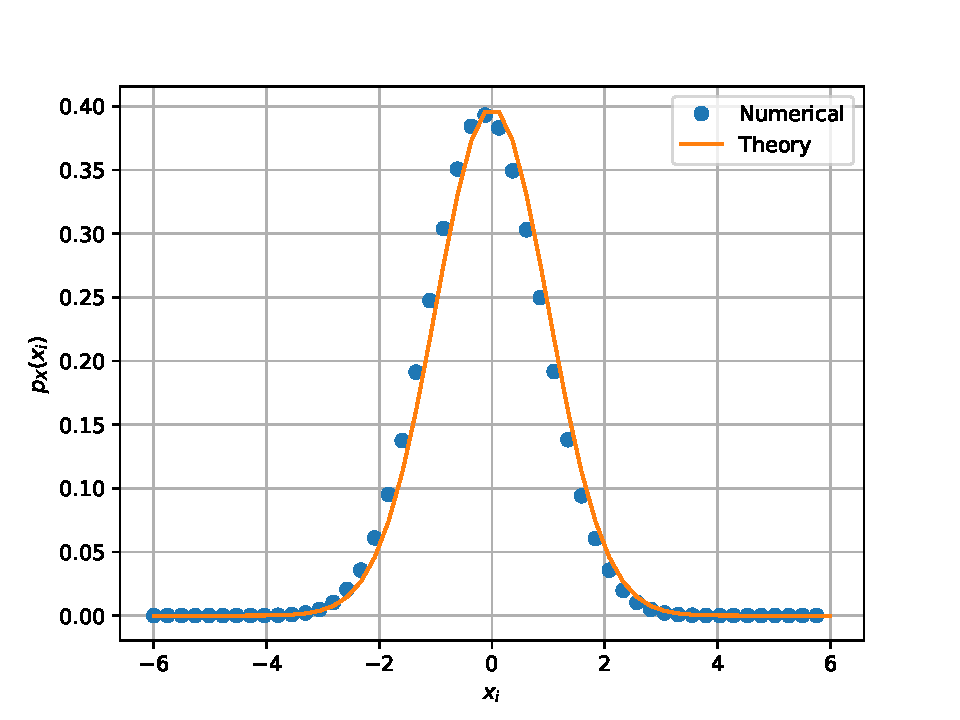
\includegraphics[width=\columnwidth]{./gauss_pdf}
\caption{The PDF of $X$}
\label{fig:gauss_pdf}
\end{figure}
\\
\solution The PDF of $X$ is plotted in \ref{fig:gauss_pdf} using the code below
\begin{lstlisting}
https://github.com/Pranavb060504/Random_numbers/blob/main/2.3/pdf.py
\end{lstlisting}
Use the below command to run the code:
\begin{lstlisting}
python3 pdf.py
\end{lstlisting}
Properties of PDF:

\begin{itemize}
\item PDF is symmetric about $x=0$\\
\item graph is bell shaped\\
\item mean of graph is situated at the apex point of the bell\\
\end{itemize}
\item Find the mean and variance of $X$ by writing a C program.\\
\solution
Running the below code gives Mean = -0.000417 Variance= 0.999902
 \begin{lstlisting}
wget https://github.com/Pranavb060504/Random_numbers/blob/main/2.4/mean_var(gau).c
\end{lstlisting}
Command used:
\begin{lstlisting}
cc mean_var(gau).c -lm
./a.out
\end{lstlisting}
\item Given that 
\begin{align}
p_{X}(x) = \frac{1}{\sqrt{2\pi}}\exp\brak{-\frac{x^2}{2}}, -\infty < x < \infty,
\end{align}
repeat the above exercise theoretically.
%
\end{enumerate}
\\
Given ,$p_{X}(x)=\frac{1}{\sqrt{2\pi}} e^{\frac{-x^2}{2}}$\\
 &E[x]=\int_{-\infty}^{\infty} x p_{X}(x) dx\\
 &=\int_{-\infty}^{\infty} \frac{1}{\sqrt{2 \pi}} x e^{-\frac{-x^2}{2}}\\
  &\because x e^{-\frac{-x^2}{2}} \text{is a odd function},\\
  \nonumber
   &E[x]=0\\
 &E[x^2]=\int_{-\infty}^{\infty} x^2 p_{X}(x) dx\\
 &=\int_{-\infty}^{\infty} \frac{1}{\sqrt{2\pi}} x(xe^{-\frac{-x^2}{2}}) dx
 \end{align}
  Using integration by parts:
  \begin{align}
   \label{eq:eq1}
 & =x\int xe^{-\frac{-x^2}{2}} dx-\int\frac{d(x)}{dx} \int xe^{-\frac{-x^2}{2}}dx\\
 &I=\int x e^{-\frac{-x^2}{2}}\\
 &\text{Let} \frac{x^2}{2}=t \\
 &\implies x dx=dt\\
 &\implies =\int e^{-t} dt=-e^{-t} +c\\
 \label{eq:eq2}
 &\therefore \int x e^{-\frac{-x^2}{2}}=-e^{-\frac{-x^2}{2}} +c
 \end{align}
 Using \eqref{eq:eq2} in \eqref{eq:eq1}\\
 \begin{align}
&= -x e^{-\frac{-x^2}{2}}+\int e^{-\frac{-x^2}{2}} dx\\
&\text{Also} ,\int_{-\infty}^{\infty} e^{-\frac{-x^2}{2}} dx=\sqrt{2 \pi} \\
&\therefore \text{substituting limits we get}, E[x^2]=1\\
 &Var(X)=E[x^2]-(E[x])^2=1-0
 \end{align}
\section{From Uniform to Other}
\begin{enumerate}[label=\thesection.\arabic*
,ref=\thesection.\theenumi]
%
\item
Generate samples of 
%
\begin{equation}
V = -2\ln\brak{1-U}
\end{equation}
%
and plot its CDF.\\ 
 \begin{figure}[h]
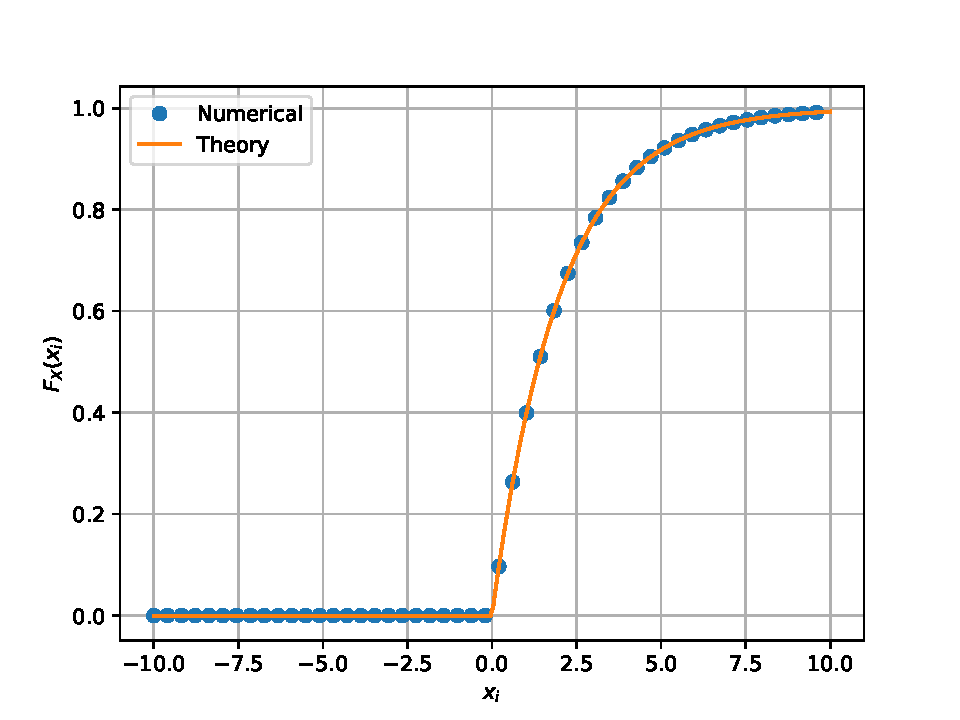
\includegraphics[width=0.5\textwidth]{V_cdf.pdf}
\caption{CDF for (3)}
\label{fig:V}
\end{figure}
\\ 
\solution
Running the below code generates samples of V from file uni.dat(U).
\begin{lstlisting}
https://github.com/Pranavb060504/Random_numbers/blob/main/3.1/V.py
\end{lstlisting}
Use the below command in the terminal to run the code:
\begin{lstlisting}
python3 V.py
\end{lstlisting}
\\ 
Now these samples are used to plot \eqref{fig:V} by running the below code,
\begin{lstlisting}
https://github.com/Pranavb060504/Random_numbers/blob/main/3.1/V_cdf.py
\end{lstlisting}
Use the below command to run the code:
\begin{lstlisting}
python3 V_cdf.py
\end{lstlisting}
\item Find a theoretical expression for $F_V(x)$.
\begin{align}
 &F_{V}(x)=P(V \leq x)\\
 &=P(-2 ln(1-U) \leq x)\\
 &=P(1-e^{\frac{-x}{2}} \geq U)\\
 &P(U<x)=\int_{0}^{x} dx=x\\
 &\therefore P(1-e^{\frac{-x}{2}} \geq U)=1-e^{\frac{-x}{2}}, \forall x\geq 0 \\ 
 \nonumber
 \end{align}
%
%\item
%Generate the Rayleigh distribution from Uniform. Verify your result through graphical plots.
\end{enumerate}
\section{Triangular Distribution}
\begin{enumerate}[label=\thesection.\arabic*
,ref=\thesection.\theenumi]
%
\item Generate 
	\begin{align}
		T = U_1+U_2
	\end{align}
\solution 
Run the below code to generate T.dat
\begin{lstlisting}
https://github.com/Pranavb060504/Random_numbers/blob/main/4.1/T_gen_dat.c
\end{lstlisting}
Run the command below in the terminal 
\begin{lstlisting}
cc T_gen_dat.c -lm
./a.out
\end{lstlisting}
\item Find the CDF of $T$.
\begin{align}
F_{T}(t)=P(T<t)
\\=P(U_1 +U_2 <t)
\end{align}
we know that $0\leq U_1 \leq 1$ and $0\leq U_2 \leq 1$\\
$\therefore 0\leq U_1 + U_2 \leq 2$, so\\
 $\forall t>2, P(U_1 +U_2 <t)=1$\\
 $\forall t<0, P(U_1 +U_2 <t)=0$\\
   for $0\leq t \leq 2$ let us split it into 2 cases, for $0 \leq t\leq 1$ and $1 <t \leq2$\\
    \begin{figure}[h]
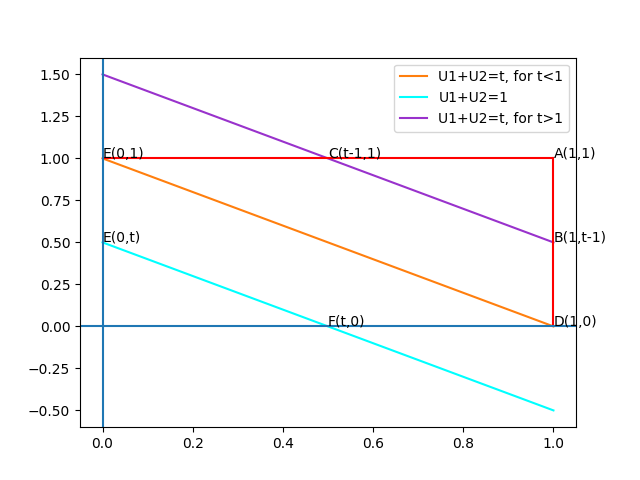
\includegraphics[width=0.5\textwidth]{T_plot}
\caption{Plot}
\label{fig:T_plot}
\end{figure}
\\
The above figure is produced by the following code
\begin{lstlisting}
https://github.com/Pranavb060504/Random_numbers/blob/main/4.2/T_plot.py
\end{lstlisting}
Run the following command in the terminal to run the code
\begin{lstlisting}
python3 T_plot.py
\end{lstlisting}
From Fig \eqref{fig:T_plot}
\begin{align}
&P(U_1+U_2<t, 0\leq t \leq 1)=\frac{ \Delta(EOF)}{\Delta(AEOD)}\\
&=\frac{t^2}{2}\\
&P(U_1+U_2<t, 1\leq t \leq 2)=\frac{\Delta(ABC)}{\Delta(AEOD)}\\
&=1-\frac{(2-t)^{2}}{2}\\
&\therefore F_{T}(t)=P(U_1 +U_2<t)=
\begin{cases}
0 & t<0\\
\frac{t^2}{2} & 0\leq t \leq 1\\
1-\frac{(2-t)^{2}}{2} & 1< t \leq 2\\
1 & t>2
\end{cases}
\end{align}
\item Find the PDF of $T$.\\
\solution 
\begin{align}
P_{T}(t)=\frac{d(F_{T}(t))}{dt}\\
\therefore P_{T}(t)=
\begin{cases}
0 & t<0\\
t & 0\leq t \leq 1\\
2-t  & 0< t \leq 2\\
0 & t>2 
\end{cases}    
\end{align}
\item Find the theoretical expressions for the PDF and CDF of $T$.
\\
\solution
\begin{align}
P_{T}(t)=
\begin{cases}
0 & t<0\\
t & 0\leq t \leq 1\\
2-t  & 0< t \leq 2\\
0 & t>2 
\end{cases} 
\\   
F_{T}(t)=
\begin{cases}
0 & t<0\\
\frac{t^2}{2} & 0\leq t \leq 1\\
1-\frac{(2-t)^{2}}{2} & 1< t \leq 2\\
1 & t>2
\end{cases}
\end{align}
\item Verify your results through a plot. 
\\
\solution 
 \begin{figure}[h]
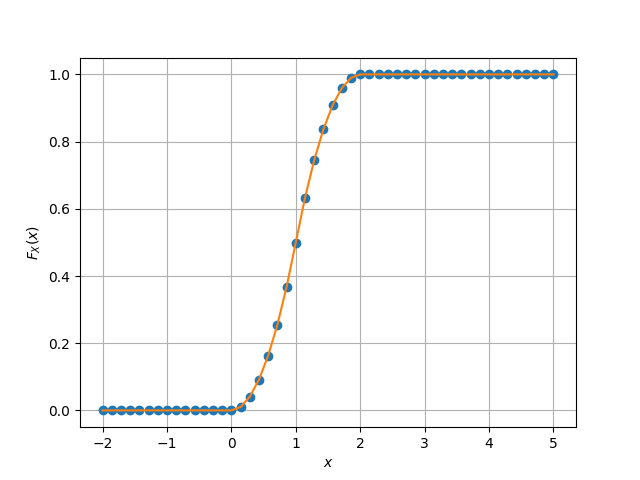
\includegraphics[width=0.5\textwidth]{T_cdf}
\caption{CDF for (4)}
\label{fig:T_CDF}
\end{figure}
Run the below code to get the cdf
\begin{lstlisting}
https://github.com/Pranavb060504/Random_numbers/blob/main/4.5/T_cdf.py
\end{lstlisting}
Use the following command in the terminal to run the code
\begin{lstlisting}
python3 T_cdf.py
\end{lstlisting}
\begin{figure}[h]
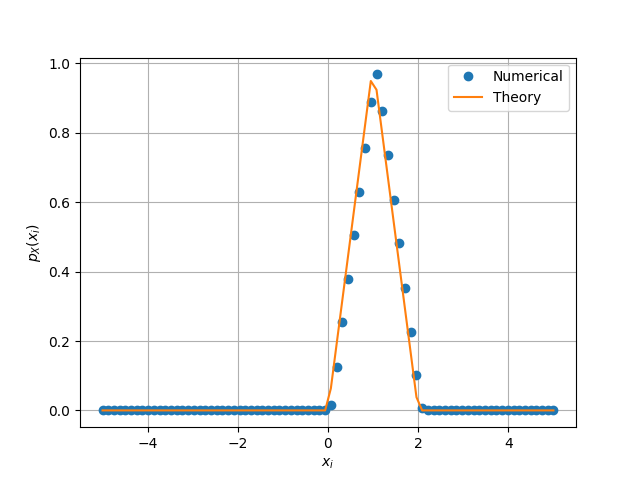
\includegraphics[width=0.5\textwidth]{T_pdf}
\caption{PDF for (4)}
\label{fig:T_PDF}
\end{figure}
Run the below code to get the pdf
\begin{lstlisting}
https://github.com/Pranavb060504/Random_numbers/blob/main/4.5/T_pdf.py
\end{lstlisting}
Use the following command in the terminal to run the code
\begin{lstlisting}
python3 T_pdf.py
\end{lstlisting}
\end{enumerate}
\section{Maximul Likelihood}
\begin{enumerate}[label=\thesection.\arabic*
,ref=\thesection.\theenumi]
\item Generate 
\begin{equation}
Y = AX+N,
\end{equation}
		where $A = 5 \text{ dB}, X \i \cbrak{1,-1}$,  is Bernoulli and $N \sim \gauss{0}{1}$.
	\item Plot $Y$.
	\item Guess how to estimate $X$ from $Y$.
\item
\label{ml-ch4_sim}
Find 
\begin{equation}
	P_{e|0} = \pr{\hat{X} = -1|X=1}
\end{equation}
and 
\begin{equation}
	P_{e|1} = \pr{\hat{X} = 1|X=-1}
\end{equation}
%
\item Find $P_e$.

%
\item
Verify by plotting  the theoretical $P_e$.  

		\end{enumerate}
\section{Gaussian to Other}
\begin{enumerate}[label=\thesection.\arabic*
,ref=\thesection.\theenumi]
\item
Let $X_1 \sim  \gauss{0}{1}$ and $X_2 \sim  \gauss{0}{1}$. Plot the CDF and PDF of
%
\begin{equation}
V = X_1^2 + X_2^2
\end{equation}
%
\solution The sum of squares of k independent standard random normal variables is nothing but a  $\chi^2$ distribution with k degrees of freedom.\\
$\chi^{2} (k)= \frac{x^{\frac{n}{2} -1}}{2^{\frac{n}{2}} \Gamma(
\frac{n}{2})} e^{\frac{-x}{2}}, \forall x\geq 0$\\
Here k=2,
\begin{align}
\therefore \chi^{2} (2)=P_{V}(v)=\frac{ e^{\frac{-x}{2}}}{2}\\
\implies F_{V}(v)=\int_{0}^{v} \frac{ e^{\frac{-x}{2}}}{2} dx\\
=1-e^{\frac{-x}{2}}
\label{eq:eq6}
\end{align}
To generate data for V , run the following code,
\begin{lstlisting}
https://github.com/Pranavb060504/Random_numbers/blob/main/6.1/V_gen.c
\end{lstlisting}
Run the below command in terminal,
\begin{lstlisting}
cc V_gen.c -lm
./a.out
\end{lstlisting}
The PDF plot of the $\chi^{2} (2)$ can be obtained by running the code below,
\begin{lstlisting}
https://github.com/Pranavb060504/Random_numbers/blob/main/6.1/chi_pdf.py
\end{lstlisting}
Use the following command in the terminal to run the code
\begin{lstlisting}
python3 chi_pdf.py
\end{lstlisting}
\begin{figure}[h]
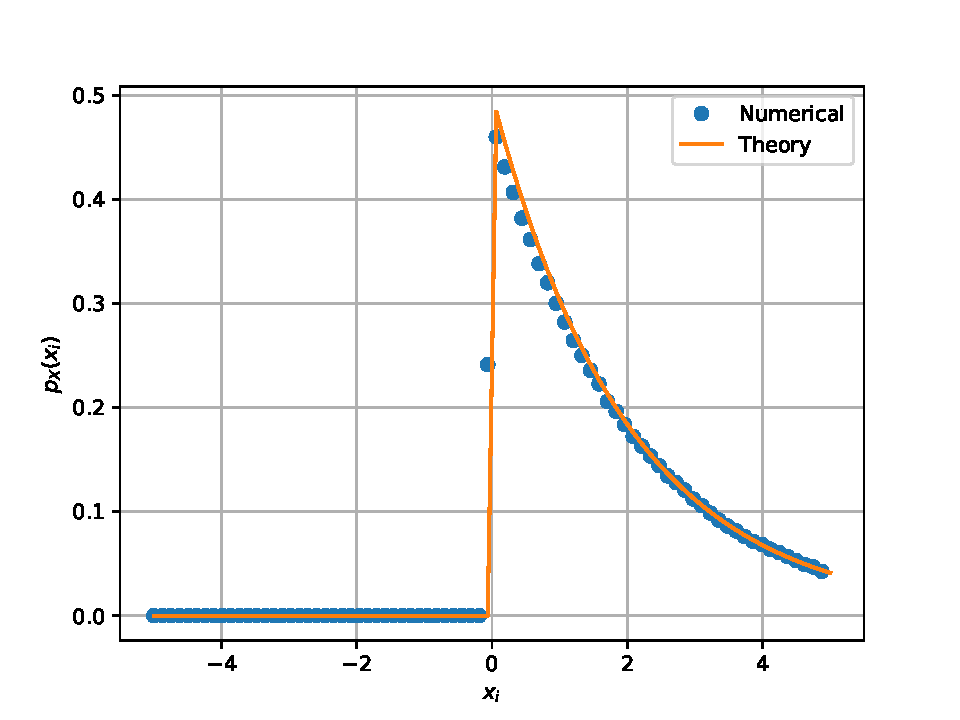
\includegraphics[width=0.5\textwidth]{chi_pdf}
\caption{PDF for (6.1)}
\label{fig:chi_PDF}
\end{figure}
The CDF plot of the $\chi^{2} (2)$ can be obtained by running the code below,
\begin{lstlisting}
https://github.com/Pranavb060504/Random_numbers/blob/main/6.1/chi_cdf.py
\end{lstlisting}
Use the following command in the terminal to run the code
\begin{lstlisting}
python3 chi_cdf.py
\end{lstlisting}
\begin{figure}[h]
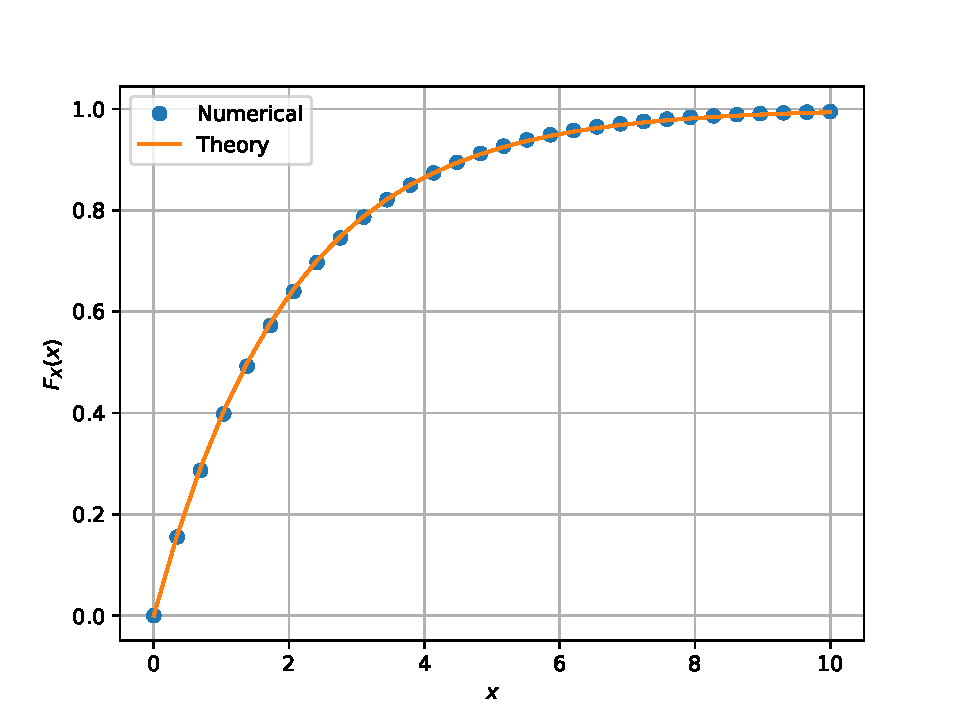
\includegraphics[width=0.5\textwidth]{chi_cdf}
\caption{PDF for (6.1)}
\label{fig:chi_PDF}
\end{figure}
%
%
%
\item
If
%
\begin{equation}
F_{V}(x) = 
\begin{cases}
1 - e^{-\alpha x} & x \geq 0 \\
0 & x < 0,
\end{cases}
\end{equation}
%
find $\alpha$.\\
\solution 
From \eqref{eq:eq6} $\alpha=0.5$

%
\item
\label{ch3_raleigh_sim}
Plot the CDF and PDf of
%
\begin{equation}
A = \sqrt{V}
\end{equation}
%
\solution
\begin{align}
&F_{A}(a)=P(A<a)=P(V<a^{2})\\
&\text{from} \eqref{eq:eq6}, 
=\begin{cases}
1-e^{\frac{-a^{2}}{2}} & a>0\\
0 & a<=0
\end{cases}
\\
&\implies P_{A}(a)= \frac{d(F_{A}(a))}{da}\\
=\begin{cases}
ae^{\frac{-a^{2}}{2}} & a>0\\
0 & a<=0
\end{cases}
\end{align}
To generate data for A , run the following code,
\begin{lstlisting}
https://github.com/Pranavb060504/Random_numbers/blob/main/6.3/A_gen.c
\end{lstlisting}
Run the below command in terminal,
\begin{lstlisting}
cc A_gen.c -lm
./a.out
\end{lstlisting}
The PDF plot of A can be obtained by running the code below,
\begin{lstlisting}
https://github.com/Pranavb060504/Random_numbers/blob/main/6.3/A_pdf.py
\end{lstlisting}
Use the following command in the terminal to run the code
\begin{lstlisting}
python3 A_pdf.py
\end{lstlisting}
\begin{figure}[h]
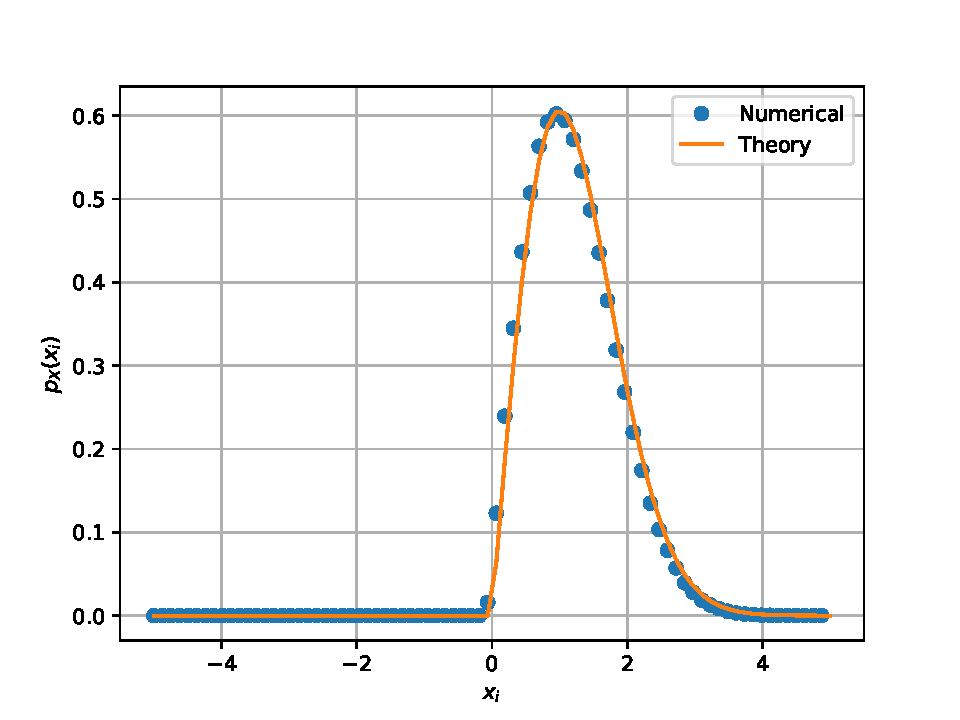
\includegraphics[width=0.5\textwidth]{A_pdf}
\caption{PDF for (6.3)}
\label{fig:A_PDF}
\end{figure}
The CDF plot of the A can be obtained by running the code below,
\begin{lstlisting}
https://github.com/Pranavb060504/Random_numbers/blob/main/6.3/A_cdf.py
\end{lstlisting}
Use the following command in the terminal to run the code
\begin{lstlisting}
python3 A_cdf.py
\end{lstlisting}
\begin{figure}[h]
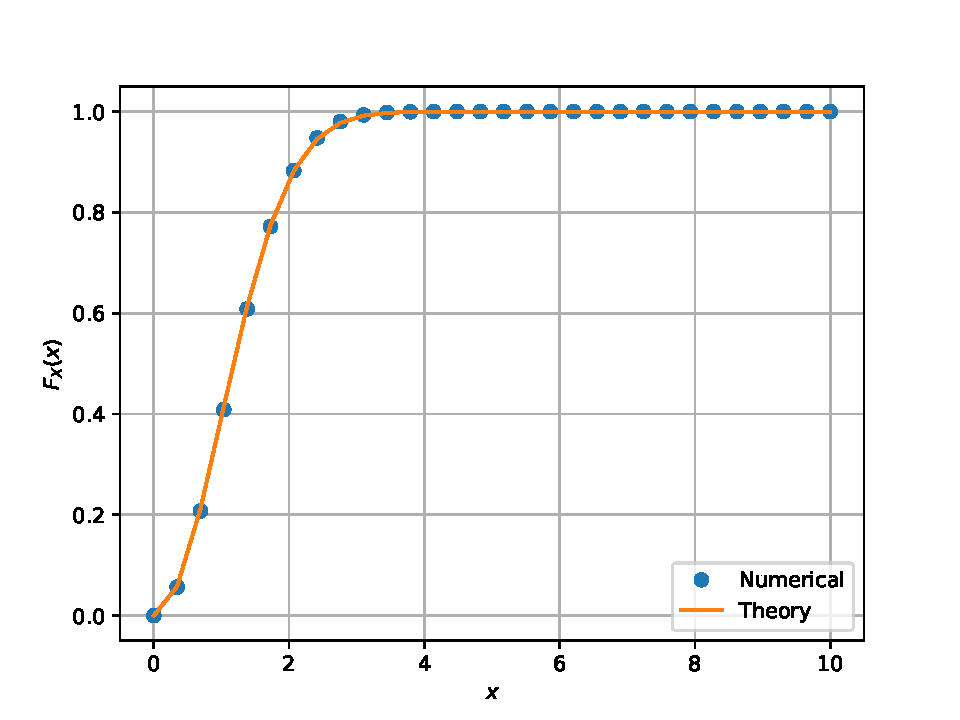
\includegraphics[width=0.5\textwidth]{A_cdf}
\caption{CDF for (6.3)}
\label{fig:A_PDF}
\end{figure}
\end{enumerate}
\section{Conditional Probability}
\begin{enumerate}[label=\thesection.\arabic*
,ref=\thesection.\theenumi]
\item
\item
\label{ch4_sim}
Plot 
\begin{equation}
P_e = \pr{\hat{X} = -1|X=1}
\end{equation}
%
for 
\begin{equation}
Y = AX+N,
\end{equation}
where $A$ is Raleigh with $E\sbrak{A^2} = \gamma, N \sim \gauss{0}{1}, X \in \brak{-1,1}$ for $0 \le \gamma \le 10$ dB.

%
\item
Assuming that $N$ is a constant, find an expression for $P_e$.  Call this $P_e(N)$

%
\item
%
\label{ch4_anal}
For a function $g$,
\begin{equation}
E\sbrak{g(X)} = \int_{-\infty}^{\infty}g(x)p_{X}(x)\, dx
\end{equation}
%
Find $P_e = E\sbrak{P_e(N)}$.

%
\item
Plot $P_e$ in problems \ref{ch4_sim} and \ref{ch4_anal} on the same graph w.r.t $\gamma$.  Comment.

		\end{enumerate}
\section{Two Dimensions}
Let 
\begin{equation}
\mbf{y} = A\mbf{x} + \mbf{n},
\end{equation}
where 
\begin{align}
x &\in \brak{\mbf{s}_0,\mbf{s}_1}, 
\mbf{s}_0 = 
\begin{pmatrix}
1 
\\
0
\end{pmatrix},
\mbf{s}_1 = 
\begin{pmatrix}
0 
\\
1
\end{pmatrix}
\\
\mbf{n} &= 
\begin{pmatrix}
n_1
\\
n_2
\end{pmatrix},
n_1,n_2 \sim \gauss{0}{1}.
\end{align}
%
\begin{enumerate}[label=\thesection.\arabic*
,ref=\thesection.\theenumi]

%%
\item
\label{ch5_fsk}
Plot 
%
\begin{equation}
\mbf{y}|\mbf{s}_0 \text{ and } \mbf{y}|\mbf{s}_1
\end{equation}
%
on the same graph using a scatter plot.

%
\item
For the above problem, find a decision rule for detecting the symbols $\mbf{s}_0 $ and $\mbf{s}_1$.

%
\item
Plot 
\begin{equation} 
P_e = \pr{\hat{\mbf{x}} = \mbf{s}_1|\mbf{x} = \mbf{s}_0}
\end{equation}
with respect to the SNR from 0 to 10 dB.

%
\item
Obtain an expression for $P_e$. Verify this by comparing the theory and simulation plots on the same graph.

%
		\end{enumerate}
\end{document}